\documentclass[12pt,a4paper,parskip]{scrartcl}
\usepackage[usenames,dvipsnames]{xcolor}
\usepackage[english]{babel}
\usepackage{titlesec}
\usepackage[usenames,dvipsnames]{xcolor}
\usepackage{libertine}
\usepackage{graphicx}
\usepackage{textcomp}
\usepackage{setspace}
\usepackage{enumitem}
\usepackage[utf8]{inputenc}
\usepackage[a4paper,left=3cm,right=3cm,top=3cm,bottom=3cm]{geometry}
\usepackage[margin=10pt,labelfont={bf},format=plain]{caption}
\usepackage[hyphens]{url}
\PassOptionsToPackage{hyphens}{url}
\usepackage[unicode,breaklinks,colorlinks=true,urlcolor=black,linkcolor=black]{hyperref}
\urlstyle{same}
\setcounter{tocdepth}{2}
\setcounter{secnumdepth}{2}
\setlength{\columnsep}{2em}
\setlist{parsep=.5em}
\titleformat{\paragraph}[hang]{\sffamily\bfseries}{\theparagraph}{.1em}{}
\titleformat{\subparagraph}[hang]{\sffamily\bfseries}{\thesubparagraph}{.1em}{}
\makeatletter\AtBeginDocument{\hypersetup{
    pdftitle={\@title},
    pdfauthor={Christian Autermann},
    pdfsubject={\@subject}
}}\makeatother
\newcommand{\mail}[1]{\href{mailto:#1}{\nolinkurl{#1}}}

\subject{\large{Environmental Modelling}}
\title{\LARGE{Exercise II: Daisyworld}}
\author{\large{Christian Autermann}\\\large{\mail{autermann@uni-muenster.de}}}
\date{\large{\today}}

\begin{document}
\maketitle
\onehalfspacing

\paragraph{1) Luminosity stays constant at 1.0}
    The population change until they find a equilibrium for the constant luminosity (see Figure~\ref{fig:temp:1}).
    After this there is no change in temperature or population (the final temperatures and populations can be found in Table~\ref{tab:temp} and~\ref{tab:population}).

\paragraph{2) A heat shock occurs: Luminosity jumps to 1.10 in 2010}
    The head shock occurs before the daisies can find a equilibrium and is compensated by a greater population of white daisies that cool the global temperature by reflecting more light (see Figure~\ref{fig:temp:2}).
    After this stable state is reached with higher temperatures than in the first scenario (the final temperatures and populations can be found in Table~\ref{tab:temp} and~\ref{tab:population}).

\paragraph{3) A cold shock occurs: Luminosity drops to 0.95 in 2010}
    The cold shocks occurs before a stable state is reached and shifts the ratio of daisies towards the black daisies.
    These are heating the global temperature by having a significant lower albedo (see Figure~\ref{fig:temp:3}).
    By this the temperature is balanced again at a lower level (the final temperatures and populations can be found in Table~\ref{tab:temp} and~\ref{tab:population}). 

\paragraph{4) Several heat shocks occur: Luminosity grows 4\% each ten years from 2010 until 2040}
    It seems, that several smaller heat shocks affect the system lesser than one big change in luminosity (see Figure~\ref{fig:temp:4}).
    The ratio between black and white daisies is not as much shifted as in scenario 2 in proportion to the change in luminosity (1.1 to $\sim$1.17) because the population of black daisies is not as much decimated by a less intrusive change in temperature.
    This results in higher population of black daisies once the system is stabilized by the white daisies in relation to the absolute change in luminosity (the final temperatures and populations can be found in Table~\ref{tab:temp} and~\ref{tab:population}).

\begin{table}
    \centering
    \begin{tabular}{l|c|c|c|c}
                      & Scenario 1 & Scenario 2 & Scenario 3 & Scenario 4\\\hline\hline
        Global        & 20.4512    & 24.9256    & 20.0245    & 25.2514 \\
        Local (White) & 15.4061    & 20.3869    & 14.4956    & 21.2545 \\
        Local (Black) & 25.4061    & 30.3869    & 24.4956    & 31.2545 \\
    \end{tabular}
    \caption{\label{tab:temp}Stable temperatures (in \textdegree C)}
\end{table}


\begin{table}
    \centering
    \begin{tabular}{l|c|c|c|c}
                      & Scenario 1 & Scenario 2 & Scenario 3 & Scenario 4\\\hline\hline
        Empty Ground  & 0       & 0       & 0       & 0       \\
        White Daisies & 495.488 & 546.131 & 447.111 & 600.307 \\
        Black Daisies & 504.512 & 453.869 & 552.889 & 399.693 \\
    \end{tabular}
    \caption{\label{tab:population}Stable populations (in ha)}
\end{table}
\begin{figure}
    \centering
    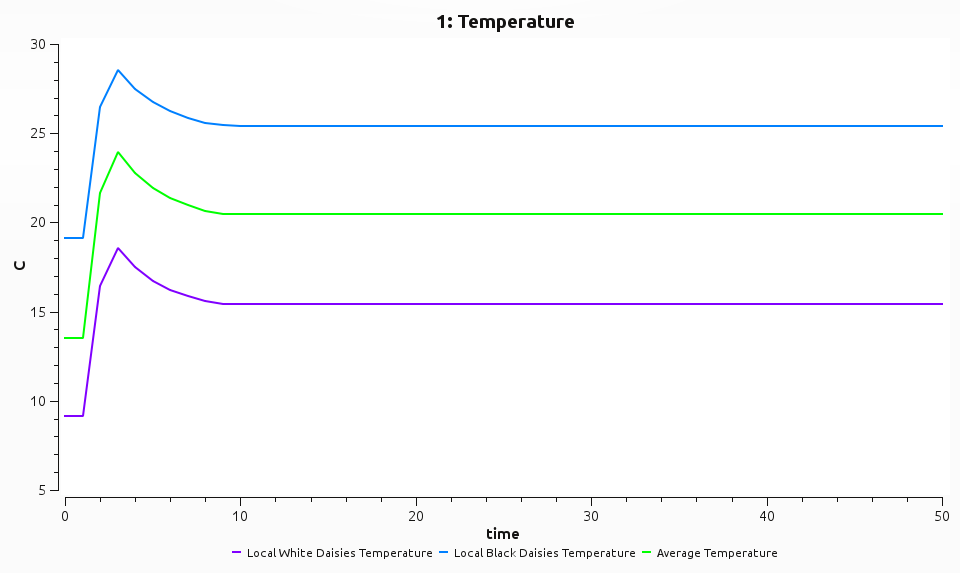
\includegraphics[width=1\textwidth]{1.png}
    \caption{\label{fig:temp:1}Temperature behavior in scenario 1}
\end{figure}
\begin{figure}
    \centering
    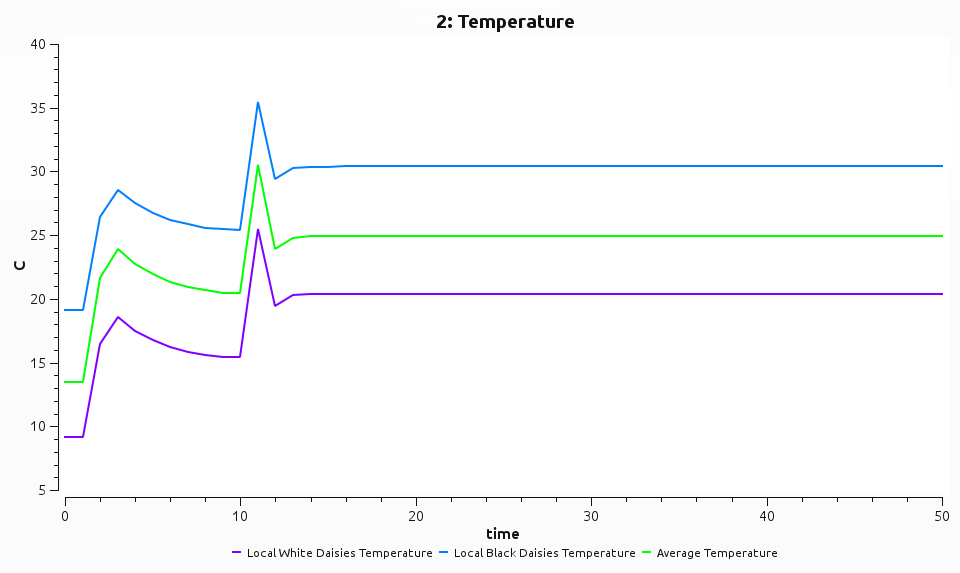
\includegraphics[width=1\textwidth]{2.png}
    \caption{\label{fig:temp:2}Temperature behavior in scenario 2}
\end{figure}
\begin{figure}
    \centering
    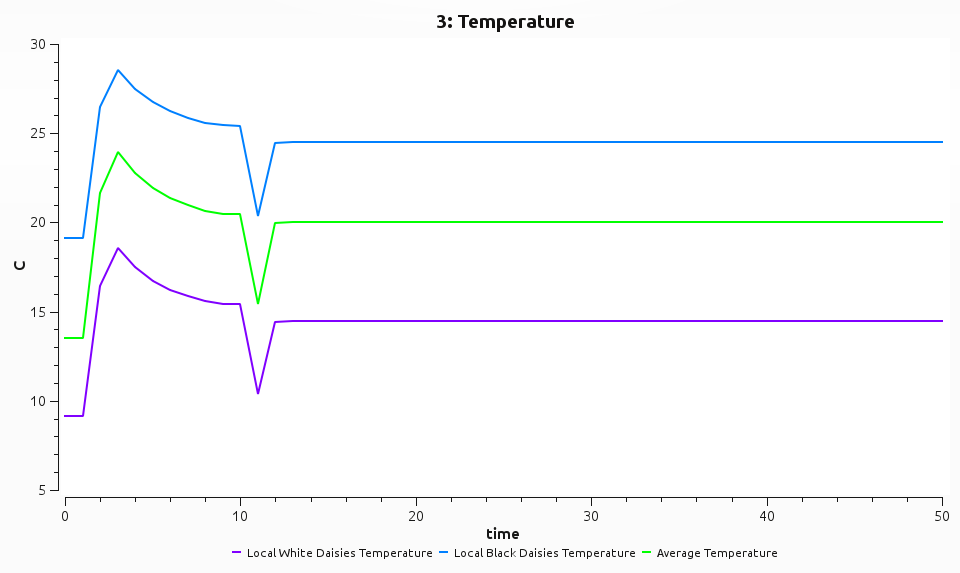
\includegraphics[width=1\textwidth]{3.png}
    \caption{\label{fig:temp:3}Temperature behavior in scenario 3}
\end{figure}
\begin{figure}
    \centering
    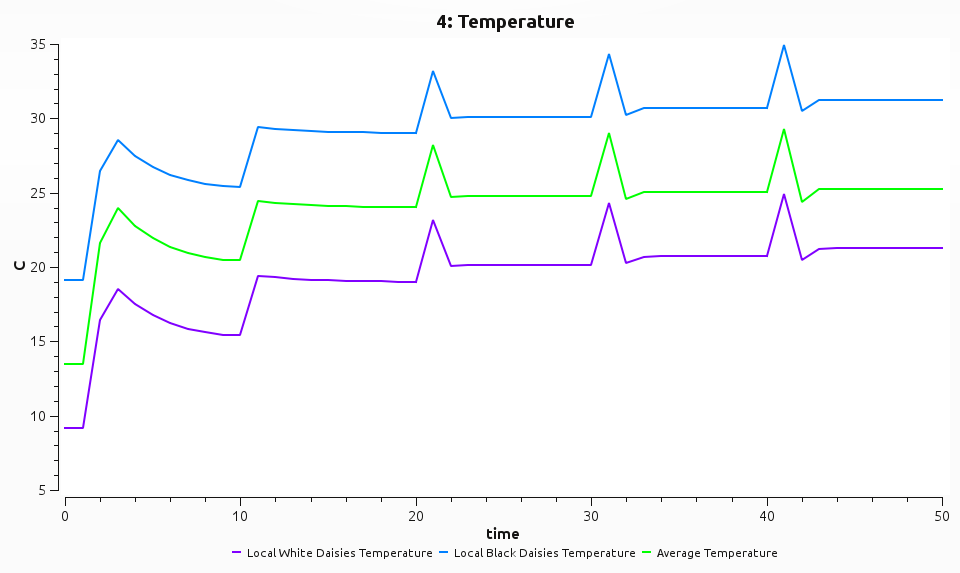
\includegraphics[width=1\textwidth]{4.png}
    \caption{\label{fig:temp:4}Temperature behavior in scenario 4}
\end{figure}
\end{document}